\chapter{Descrição Geral do Sistema }

Este capítulo tem como objetivo descrever de forma geral o sistema, o escopo e as principais funções. A descrição geral do sistema deve abrange os itens a seguir: descrição do problema que o software terá que resolver, seus envolvidos e suas características para implementação de cada função na solução.

%Este capítulo tem como objetivo descrever de forma geral o sistema, o escopo e as
%principais funções. A descrição geral do sistema deve abrange os itens a seguir: descrição do problema que nosso software terá que resolver, seus envolvidos e suas características para desenvolver cada função no desenvolvimento da solução como de seus usuários e regras de negocio que serão implementadas nessa primeira versão.
%Um sistema de gerenciamento de ordens de serviços ,com consulta em estoque .
% ---
\section{Descrição do Problema}
% ---
O desenvolvimento deste sistema, tem como objetivo resolver principalmente os problemas a seguir:
%O desenvolvimento deste sistema, tem como objetivo resolver principalmente os problemas a seguir:

\begin{itemize}
	\item Fluxo lento nos processos de manutenção industrial na empresa
	\item Falta de automação
	\item Logística complicada
	\item Falta de Controle das informações
	\item Dificuldade em armazenar informações
	%\item

\end{itemize}

%O software Smart Solution terá como diferencial tornando possível os itens a seguir:

O software \textit{Smart Solution} terá como diferencial tornar possível os itens a seguir:

\begin{itemize}

	\item Transformar o processo de manutenção em um processo digital de fácil controle
	\item Gerenciar as ordens de manutenção
	\item Transformar os apontamentos de produção dos mecânicos rápido e dinâmico.
		
\end{itemize}

O sistema irá afetar diretamente a equipe de manutentores da empresa, que poderão reduzir a sua carga de trabalho e focar em outras atividades mais produtivas. Para que haja uma boa relação de usuário com o sistema, será desenvolvido uma aplicação mobile, e o sistema permitirá o pedido de peças para o estoque de uma maneira simples.
%O sistema irá afetar diretamente a equipe manutentores da empresa Duas Rodas, que poderão reduzir a sua carga de trabalho e focar em outras atividades mais produtivas.
%Para que haja uma boa relação de usuário com o sistema, será densenvolvido uma aplicação mobile, e o sistema permitira o pedido de peças para o estoque de uma maneira simples.
% ---
\section{Principais Envolvidos e suas Características}
% ---
% ---
\subsection{Usuários do Sistema}
% ---
%O sistema será desenvolvido para uma empresa do setor Industrial, mais especificamente para o setor de mecânica, logo os principais usuários serão os mecânicos e o líder do setor da mecânica.
O sistema será desenvolvido para uma empresa do setor Industrial, mais especificamente para o setor de mecânica, logo os principais usuários serão os mecânicos e o líder do setor da mecânica.
% ---

\subsection{Desenvolvedores do Sistema}
% ---
%Os desenvolvedores do sistema serão os alunos curso de Sistemas para Internet da instituição SENAI Jaraguá do Sul. Além disso os professores das disciplinas curriculares do curso, participarão ativamente das atividades necessárias para o desenvolvimento, auxiliando tecnicamente e coordenando as equipes, para que os projeto possam fluir da maneira mais adequada. O projeto também conta com um coordenador, que é o principal responsável pelo projeto.
Os desenvolvedores do sistema serão os alunos do curso de Sistemas para Internet da instituição SENAI Jaraguá do Sul. Além disso os professores das disciplinas curriculares do curso, participarão ativamente das atividades necessárias para o desenvolvimento, auxiliando tecnicamente e coordenando as equipes, para que os projetos possam fluir da maneira mais adequada. O projeto também conta com um coordenador, que é o principal responsável pelo projeto.
% ---
\section{Método PMBOK }
% ---
O PMBOK e um guia que reuni a soma dos conhecimento e boas práticas de gerencia em gerência de projetos, que pode ser utilizada em todas as áreas do conhecimento."A primeira versão do PMBOK foi criada em 1986 e a versão atual é de 2017. Ela foi gerado pelo PMI - Project Management Institute que é uma associação de profissionais de gerência de projetos e existe desde 1969."\cite{machado2001gerencia}.

Segundo \cite{maciel2006metodo} o PMBOK padronizou para cada etapa do projeto diversos processos com o objetivo de produzir o resultado esperado de cada etapa, ou seja, os processos ocorrem em todas as etapas do projeto, e dependendo da etapa que estiver poderá haver maior incidência de processos. 
%e explica com referencias PMBOK

% ---------
\subsection{Fluxo de processos}
 O Fluxo de processos PMBOK abrange 10 áreas de conhecimento, cinco grupo de processos e possui 49 processos na sua estrutura.\cite{borja2019aplicaccao}. Dentro dessas 10 áreas do conhecimento do fluxo de processos, será utilizado neste projeto 8 deles que são: integração, escopo, cronograma, qualidade, recursos, comunicações, riscos, partes interiçadas. Que está ilustrado na imagem abaixo:
 

% ----
\begin{figure}[H]
	\caption{\label{fluxo_de_processos_PMBOK}Fluxo de processo da \textit{Smart Solution}}
	\centering
	\mbox{%
		{
			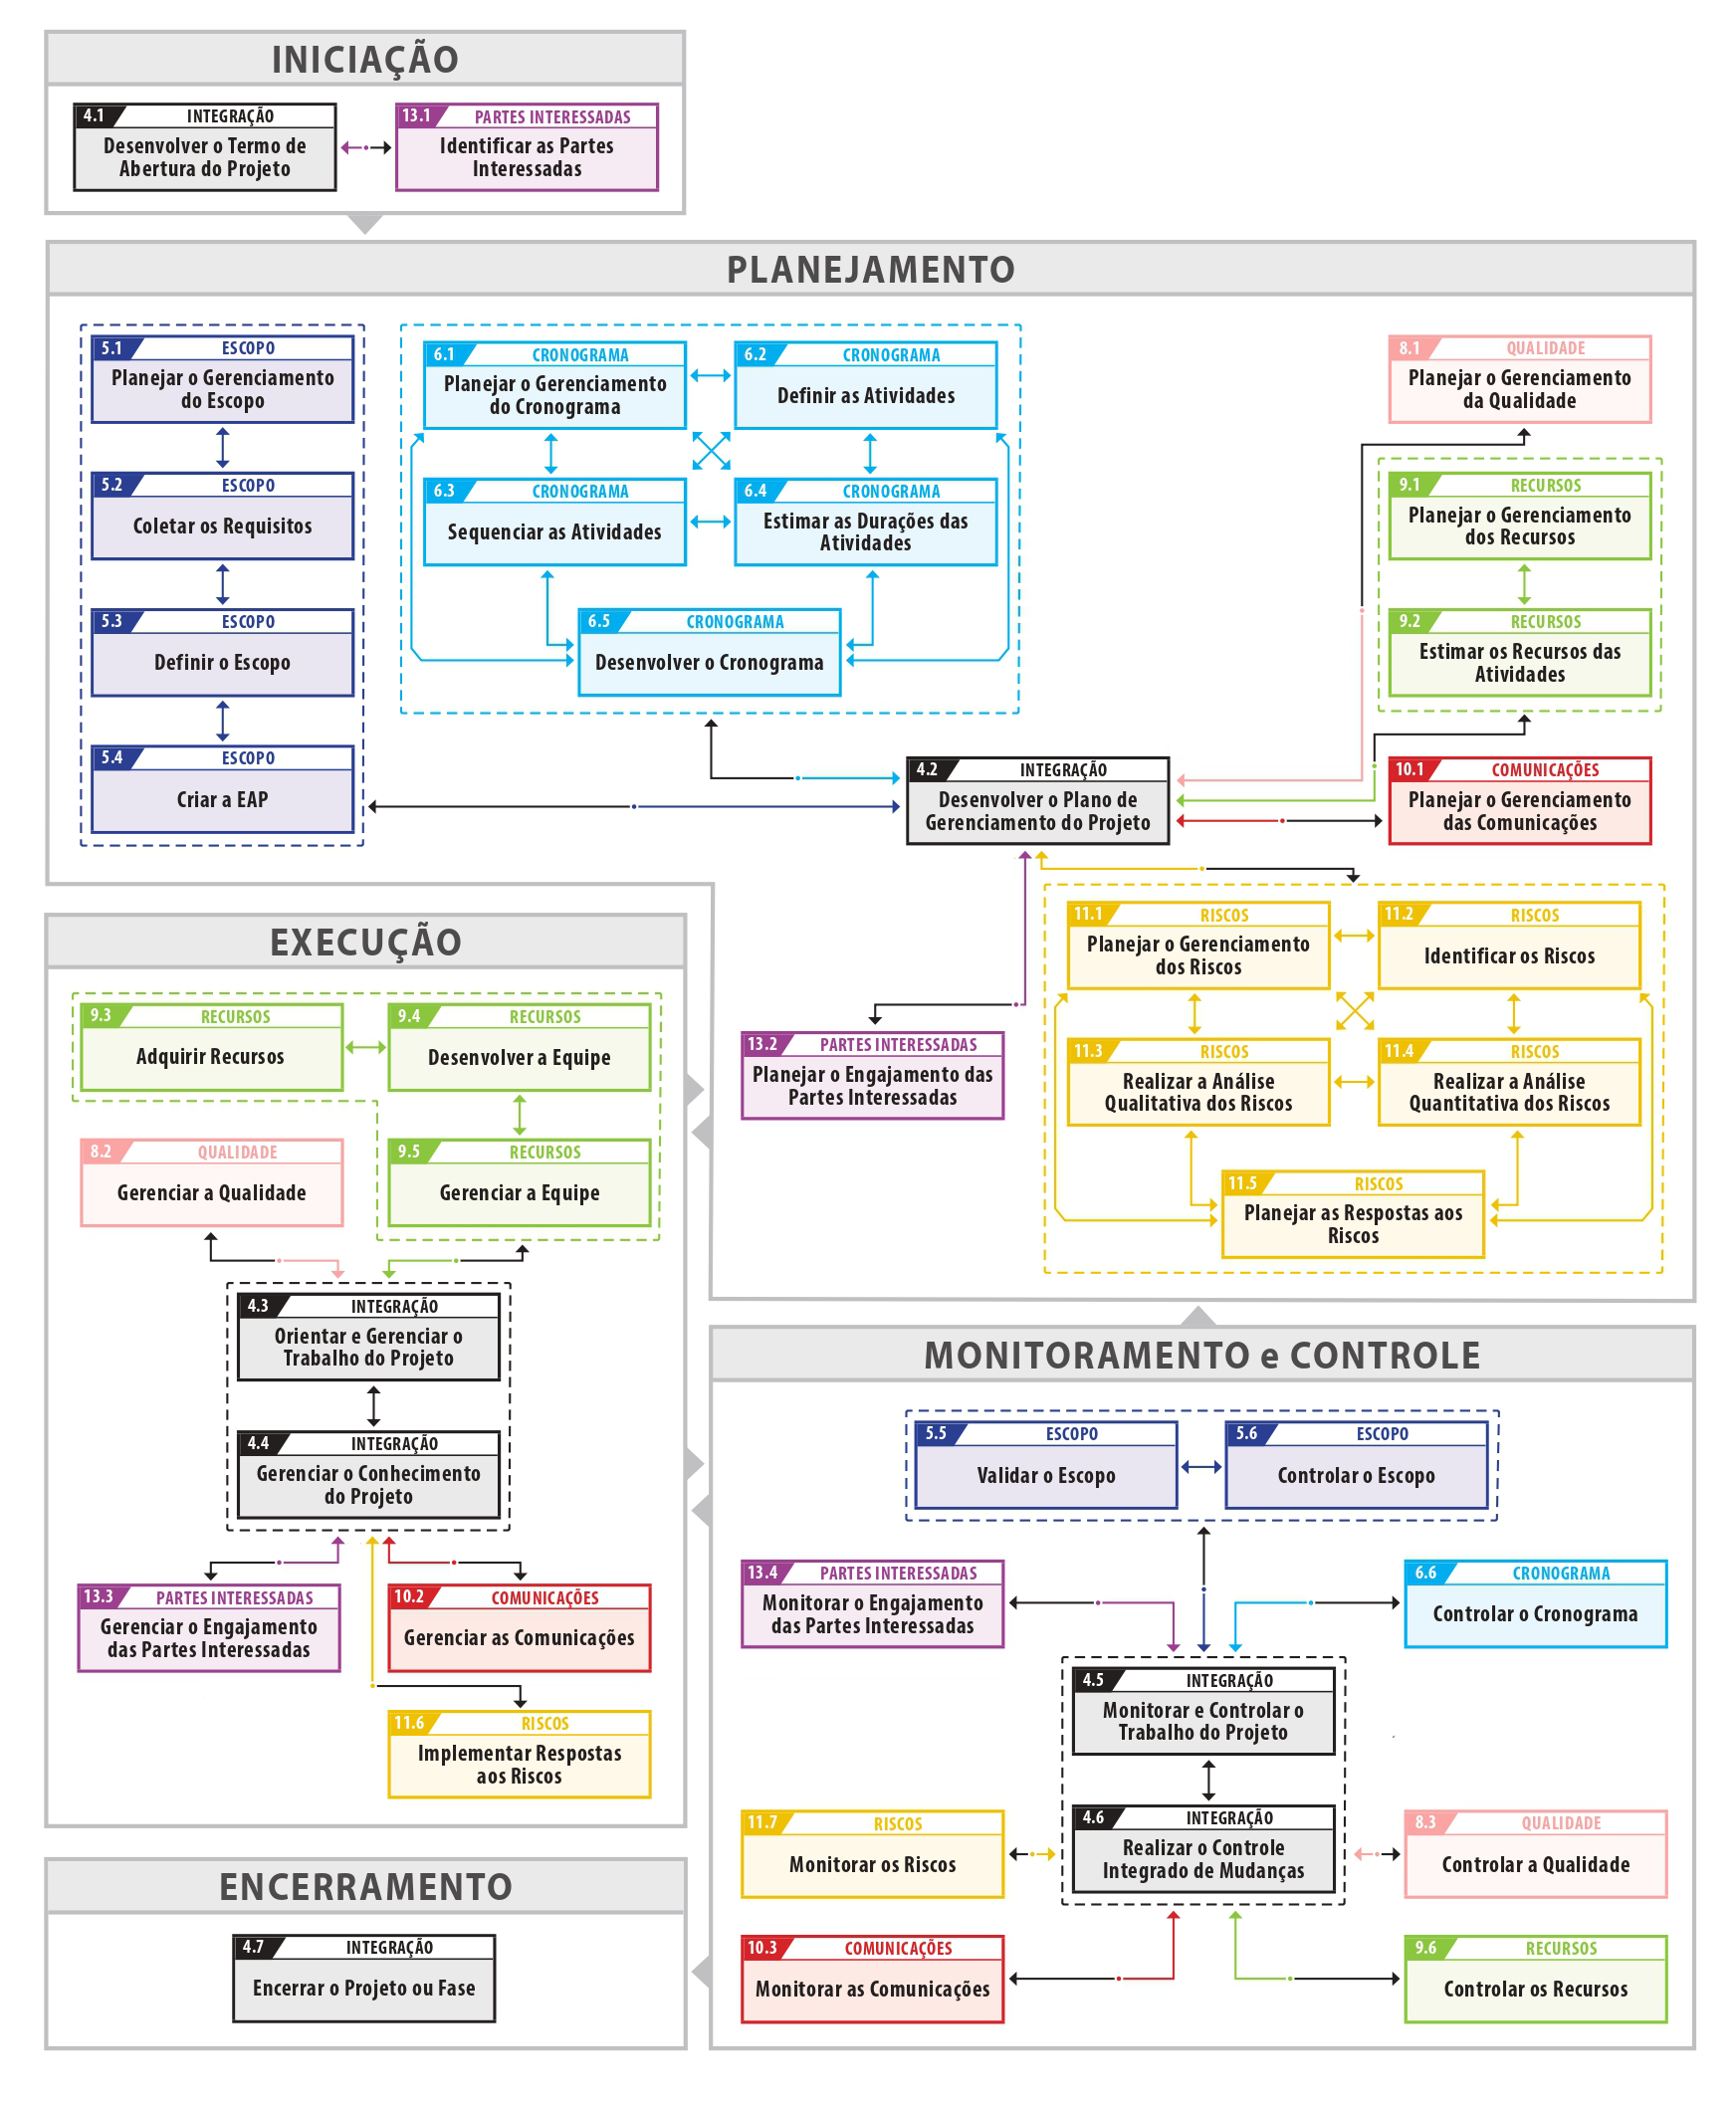
\includegraphics[scale=0.62]{Figuras/fluxo_de_processos_PMBOK}}\qquad
		
	}
	
	
\end{figure}

% ----
\subsection{EAP}
% ----
O EAP e uma estrutura de forma visualizar as atividades que compõem o projeto, permitindo visualizar todo o escopo do projeto. Onde no topo fica o projeto, na segunda camada fica as etapas que no EAP e chamada de entregáveis, e para cada entregável possui as subcamadas que são as tarefas necessárias para finalizar cada uma das etapas do desenvolvimento. Na imagem abaixo mostra o EAP desenvolvido para o projeto \textit{Smart Solution}.

\begin{figure}[H]
	\caption{\label{EAP_Smart_Solution4}EAP da \textit{Smart Solution}}
	\centering
	\mbox{%
		{
			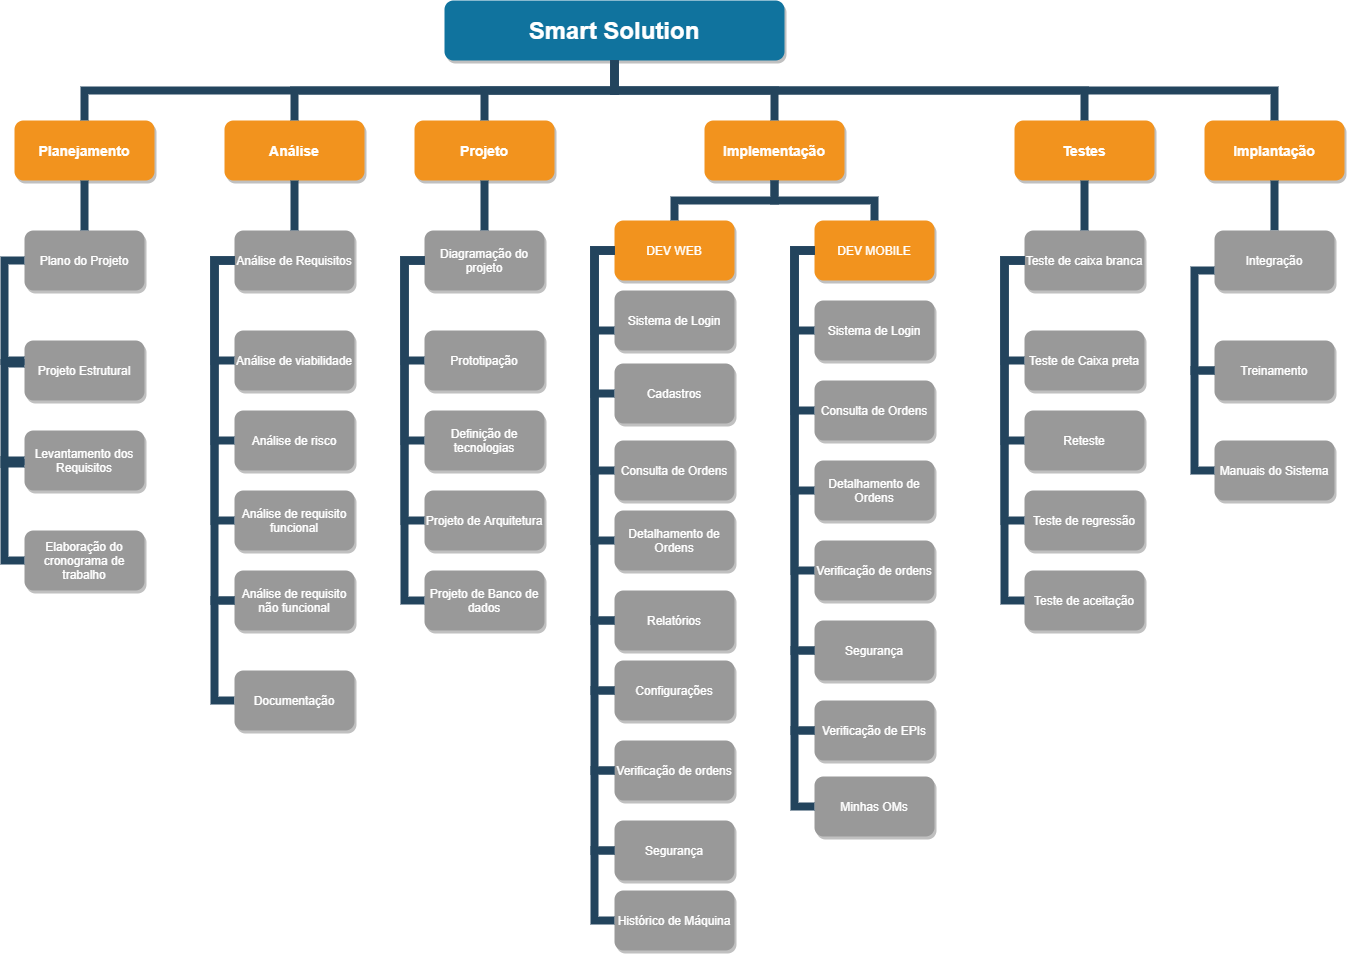
\includegraphics[scale=0.47, angle=90]{Figuras/EAP_Smart_Solution4}}\qquad
		
	}
	
	
\end{figure}
% -----

\section{Regras de Negocio}
% ---

%Para o desenvolvimento do sistema os envolvidos deveram estar cientes que o sistema deverá ser integrado ao Sistema SAP, que irá enviar os dados da Ordem de Manutenção, o sistema a ser desenvolvido deverá conseguir inserir esses dados em seu Banco de dados, que obrigatoriamente fará a utilização do SQL Server. Algumas das validações que serão implementadas são: A assinatura eletrônica por meio do crachá e validações para determinar se o usuário existe no sistema ou erros de acesso. (ALTERAR)

%falta definiçao cioentifica
Pode se definir regra de negócio como sendo uma norma, ou um uso comum que determina a forma de realização de uma transação que envolve uma determinada organização.\cite{alvarenga2007abordagem}

Sempre que uma ordem de serviço for gerada no SAP para a manutenção, esta será integrada e armazenada no sistema próprio de ordem de serviços do setor da manutenção, cada OS gerada deverá ter um tipo de manutenção a ser realizado, esta pode ser preditiva, preventiva, rotas ou listas, toda OS que for gerada pelo sistema SAP deverá ter um responsável atribuído no sistema, apenas este e o administrador geral do sistema terão acesso total a ordem de serviço.
Na tela “Minhas OS”, o manutentor terá acesso as ordens que foram delegadas ao mesmo com essa ele poderá acessar mais detalhes de os, tanto para obter mais informações do serviço a ser realizado, como também ter a capacidade de realizar modificações na ordem, podendo lançar as horas trabalhadas, e organizar as operações a serem realizadas.

Quando um manutentor necessitar solicitar uma peça para o almoxarifado, este deverá acessar a tela de solicitação de peças e realizar a solicitação, está será enviada para o almoxarifado.
Quando um manutentor decidir iniciar uma ordem de serviço, ele deverá na tela “Minhas Os” acessar a aba abertas, então escolher a ordem que deseja iniciar. Se o manutentor decidir pausar a ordem, ele deverá ir até a aba em andamento e escolher a ordem que deseja pausar.
Se o manutentor terminar o serviço a ser realizado, ele deverá ir até a tela de verificação que pode ser acessada através da tela de “detalhe de ordem de serviço”, e nessa tela ele irá realizar a verificação da ordem de serviço, para a verificação ser realizada será necessária a verificação do serviço por do solicitante e do manutentor que se responsabilizou estas podem ser realizadas na tela de verificação do sistema Mobile, o manutentor também deverá preencher informações sobre o fim da OS, como solução realizada, e informar se o serviço foi finalizado, após isso a ordem deve ser analisada pelo administrador do sistema, no sistema web, ele irá decidir se a ordem deve ser encerrada ou reaberta, para ser refeita.
O Administrador do sistema poderá através da tela de detalhe da ordem de serviço, delegar mais responsáveis em uma OS.
O Administrador do sistema terá a possibilidade de acessar a tela de relatórios, nela será possível analisar o desempenho do setor de manutenção.
O administrador poderá através do sistema web acessar uma tela de notificações.
O Administrador poderá acessar e cadastrar novos centro de custo, causa de defeito,
sintoma de defeito, tipo de máquina, componente, equipamento.

\newpage

O administrador poderá acessar a tela de histórico de OS, nela será possível verificar modificações nos status da os.

Tanto o Manutentor quanto o administrador poderão acessar a tela de “Consulta de ordens”, nela será possível realizar filtros para encontrar ordens de serviço especificas.

O manutentor poderá cadastrar manualmente OS, de três tipos corretiva, preventiva, rotas e listas.

Sempre que um mecânico iniciar uma ordem de serviço será verificado os EPIs que o mesmo está utilizando, o manutentor deverá informar quais EPIs o mesmo está utilizando.
Se o manutentor pausar uma ordem, quando ele voltar, terá de preencher o Checklist de EPIs novamente informando quais EPIs ele está utilizando no momento.

O administrador poderá cadastrar novas parametrizações de segurança.
Os manutentores terão acesso aos detalhes de todas as ordens de serviço, de forma que os mesmos possam visualizar as informações pertinentes as ordens de serviço, porém sem poder realizar modificações ou alterações nas ordens de serviço que não estejam delegas para si próprio.

O administrador terá a capacidade de cadastrar tipos de operações predefinidas pela empresa, a mesmas serão utilizadas nas ordens de serviço pelos manutentores para facilitar o esboço do trabalho a ser realizado. 





\begin{figure}[H]
	\caption{\label{regraSimples1}Regras de Negócio Simplificada Parte 1 Da \textit{Smart Solution}}
	\centering
	\mbox{%
		{
			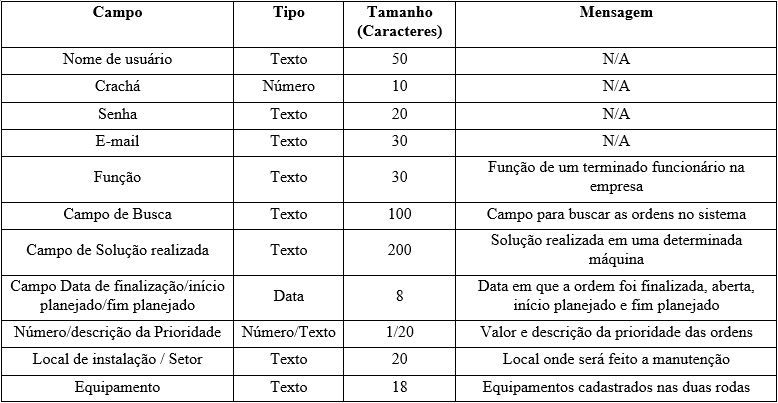
\includegraphics[scale=0.82]{Figuras/regraSimples1}}\qquad
		
	}
	
	
\end{figure}
\begin{figure}[H]
	\caption{\label{regraSimples2}Regras de Negócio Simplificada Parte 2 Da \textit{Smart Solution}}
	\centering
	\mbox{%
		{
			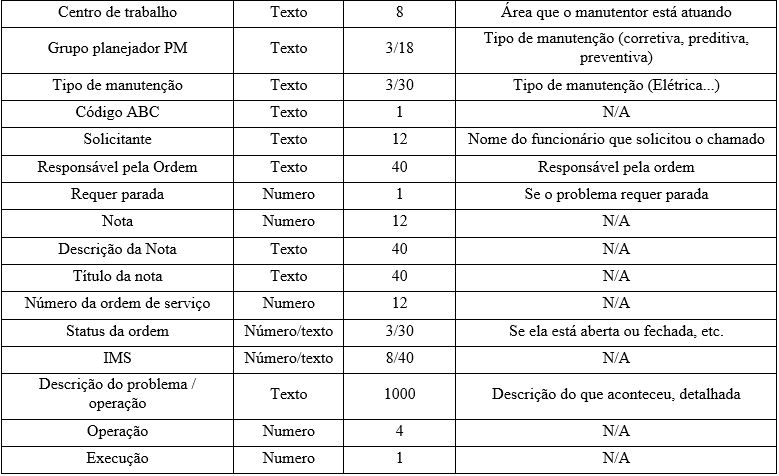
\includegraphics[scale=0.82]{Figuras/regraSimples2}}\qquad
		
	}
	
	
\end{figure}
\begin{figure}[H]
	\caption{\label{regraSimples3}Regras de Negócio Simplificada Parte 3 Da \textit{Smart Solution}}
	\centering
	\mbox{%
		{
			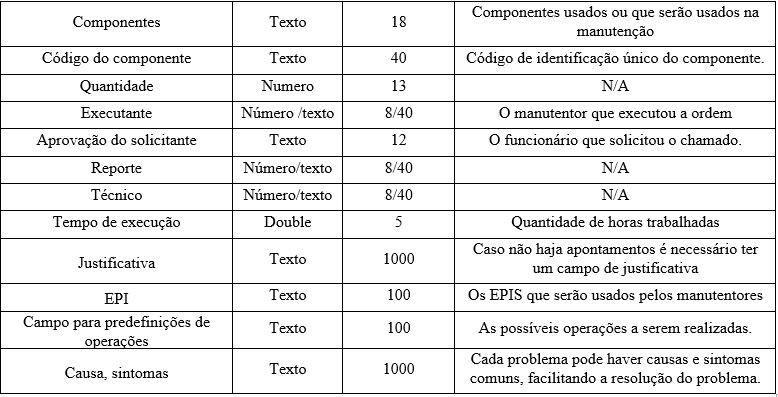
\includegraphics[scale=0.82]{Figuras/regraSimples3}}\qquad
		
	}
	
	
\end{figure}

% ---



\newpage
\section{Riscos do Projeto}
% ---
O risco em um projeto de software é uma medida da probabilidade e da perda
relacionadas à ocorrência de um evento negativo que afete o próprio projeto, seu
processo ou o seu produto. Em outras palavras, qualquer coisa que possa acontecer e
ameaçar o bom andamento do projeto é um risco. O risco do projeto relaciona-se com
aspectos operacionais, organizacionais e contratuais. Este tipo de risco é uma
responsabilidade do Gerente do Projeto, nele estando incluídos limitações de
recursos, interfaces externas, relacionamentos com fornecedores e restrições
contratuais.\cite{aguiar2011gerenciando}


\begin{figure}[H]
	\caption{\label{Tabelas_riscos}Tabela de riscos do projeto \textit{Smart Solution}}
		\centering
		\mbox{%
			{
		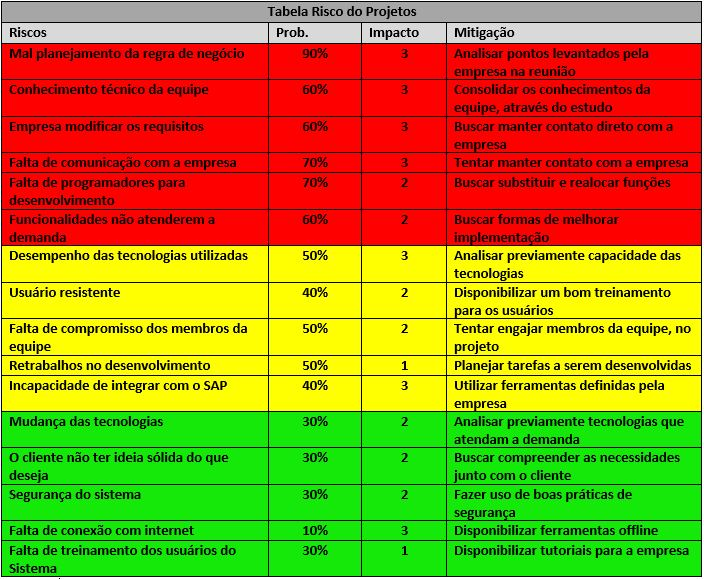
\includegraphics[scale=0.91]{Figuras/Tabelas_riscos}}\qquad
	
		}


\end{figure}

% ----
\section{Diagrama de Causa e Efeito}
% -----
O diagrama de causa e efeito ou espinha de peixe, e utilizado para estruturar causas para um determinado efeito e encontra as áreas onde podem ser introduzido melhorias, mais também pode ser utilizado controlar o processo e garantir qualidade no produto final, assim como relacionar um defeito com as suas causas. Neste projeto será utilizado esse diagrama para localizar as possíveis problemas que podem afetar o processo de desenvolvimento e conclusão do desenvolvimento do software. Na figura abaixo mostra o diagrama de causa e efeito da \textit{Smart Solution}.

\begin{figure}[H]
	\caption{\label{smart_solution_espinha_de_peixe}Diagrama de Causa e Efeito da \textit{Smart Solution}}
	\centering
	\mbox{%
		{
			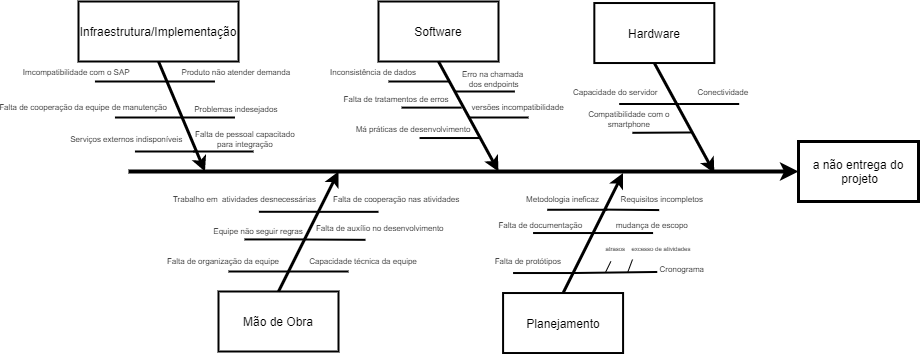
\includegraphics[scale=0.70, angle=90]{Figuras/smart_solution_espinha_de_peixe}}\qquad
		
	}
	
	
\end{figure}

% ---